\section{Execution Unit}
The Execution Unit is the unit responsible for the computations and the general execution of the commands.
The core and most significant component is the ALU, which the Execution Unit simply surrounds with multiplexers
and their controller to select the operands.

\begin{figure}[htbp]
    \center
	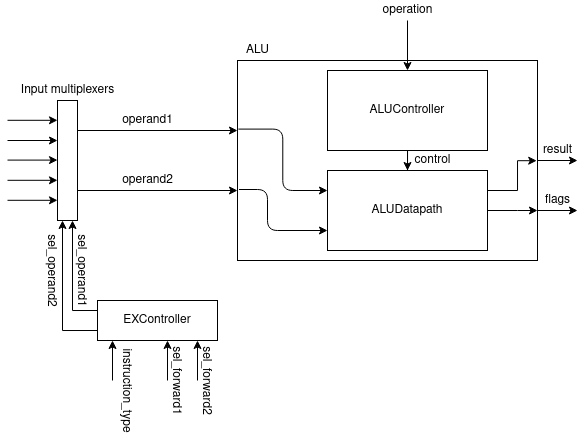
\includegraphics[width=0.8\textwidth]{./2-implementation/images/ExStage.png}
	\caption{Block view of the execution stage}
	\label{fig:exstage}
\end{figure}

\subsection{ALU}
The ALU is also internally organized with a datapath and its own controller. It is important to underline that to not
interfere with the processor's pipeline, this controller (as well as the Execution Stage's) is fully combinational and
mostly acts as an input translator.

\subsubsection{Datapath}
The datapath instantiates the arithmetic and logic operators, generates the status flags and outputs the final result.
All the operators are instantiated in parallel and, at every cycle, they all run their own operation and the result
is selected through a multiplexer. If power consumption is to be considered, guarded evaluation can be a simple
solution to optimize this behavior.

The available operators are:
\begin{itemize}
    \item Carry Look Ahead adder
    \item Barrel shifter
    \item And
    \item Xor
    \item Comparator
\end{itemize}

Most of the functionalities are straightforward: the \texttt{and} and \texttt{xor} operators are simple logic gates and
the barrel shifter is described through the \texttt{numeric\_std} library's function \texttt{shift\_right}.
The components worth discussing are the adder and the comparator.

\paragraph{Adder}
The adder is designed as a \textbf{Ladner-Fischer} Carry Look Ahead.
\begin{figure}[htbp]
    \center
	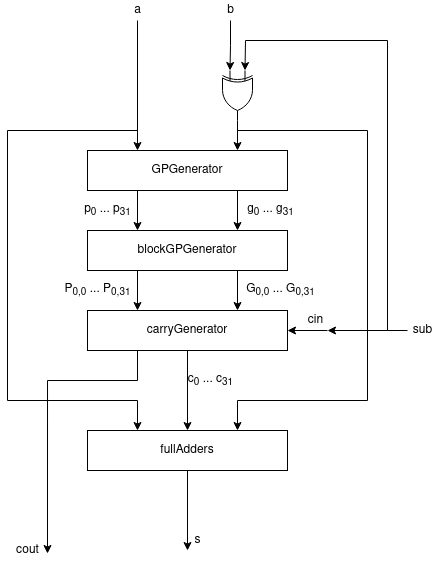
\includegraphics[width=0.5\textwidth]{./2-implementation/images/AdderCLADiagram.png}
	\caption{Carry Look Ahead adder organization}
	\label{fig:adder-diagram}
\end{figure}
Its structure is organized as a cascade of the following functional blocks:
\begin{enumerate}
    \item Sign converter \\
    To accomodate for subtractions, operator \signal{b} goes through a \texttt{xor} gate controlled by the
    \texttt{sub} signal which, when asserted, inverts \signal{b} and sets \signal{cin} to 1.

    \item Generate and Propagate bits generator \\
    Given \signal{a} and \signal{b}, output the corresponding generate and propagate signals bit by bit, where
    \begin{align*}
        g_i &= a_i\ \texttt{and}\ b_i \\
        p_i &= a_i\ \texttt{xor}\ b_i
    \end{align*}

    \item Block Generate and Propagate bits generator \\
    Starting from $g_i$ and $p_i$, compute the block generate $G_{0, i}$ and propagate $P_{0, i}$ as a parallel prefix
    problem. This is where the Ladner-Fischer structure is instantiated.

    \begin{figure}[htbp]
        \center
    	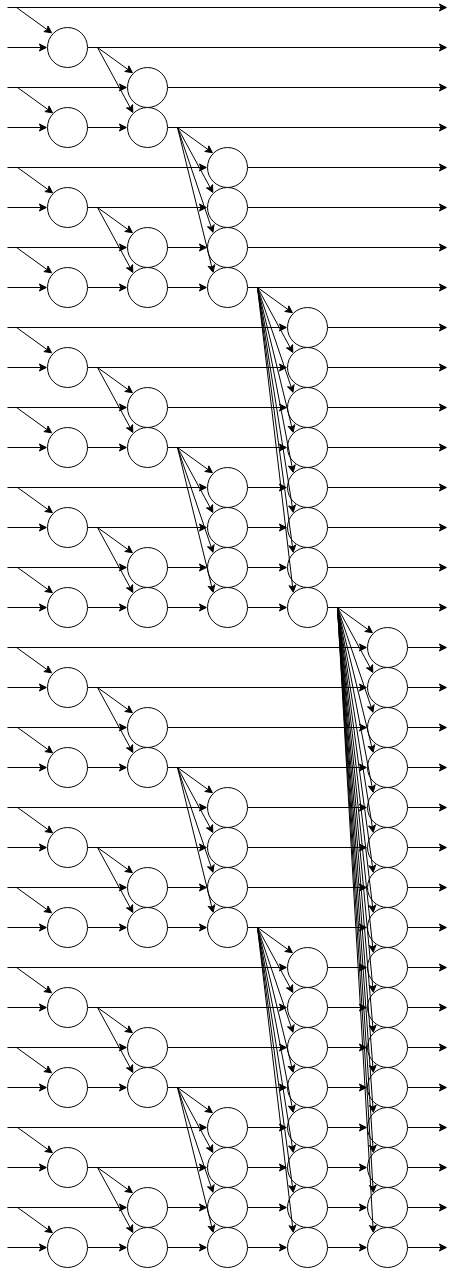
\includegraphics[width=0.5\textwidth]{./2-implementation/images/LadnerFischer.png}
    	\caption{Ladner-Fischer GPCombiner. Each circle represents an instance of the component GPCombiner.}
    	\label{fig:LadnerFischer}
    \end{figure}
    The main component needed to compute the block generate and propagate is called \texttt{GPCombiner} which, given
    $P_{i, j}$ and $P_{j, k}$, combines them into $P_{i, k}$ - the same goes for $G$. The inputs $g_i$ and $p_i$
    (lowercase, meaning they are bit-wise and not block-wise) are assumed as $G_{i, i}$
    and $P_{i, i}$, which is equivalent. The operation is simple:
    \begin{align*}
        G_{i, k} &= G_{j, k}\ \texttt{or}\  \left( G_{i, j}\ \texttt{and}\ P_{j, k} \right) \\
        P_{i, k} &= P_{i, j}\ \texttt{and}\ P_{j, k}
    \end{align*}
    The combiners are interconnected according as in the schematic in \autoref{fig:LadnerFischer} in a module
    called \texttt{blockGPGenerator}. To keep the generality of the component, the block is described with generics
    and its structure is instantiated \textbf{recursively}. More information on the VHDL description can be found in
    \autoref{appendix:recursive-adder-description}.

    This is the slowest stage since paths of different bit weight are interconnected and they form a cascade.
    The choice of the Ladner-Fischer architecture makes so that the introduced delay is $\log_2{N}$.

    \item Carry Generator \\
    Given the results from the previous stage, it is possible to compute the value of all $c_i$ in parallel, since
    \begin{align*}
        c_i &= G_{0, i}\ \texttt{or}\ (c_0\ \texttt{and}\ P_{0, i})
    \end{align*}

    \item Full adders \\
    The final stage is a barrier of full adders. At this point, every adder has all of its inputs ready: $a_i$, $b_i$,
    $c_i$. For this reason there is no need for one adder to wait for the result of another adder, so they can all
    operate in parallel, so the introduced delay is only $1\ ^t\text{FA}$.

    \item Flag generators \\
    The adder also generates two overflow flags to be used to control the flow of operations: one for signed sums, one
    for unsigned ones. In particular,
    \begin{align*}
        \texttt{cout} = C &= c_{32} \\
        \texttt{ovf} = V &= c_{32} \texttt{ xor } c_{31}
    \end{align*}
\end{enumerate}
The ALU also internally computes all of the status flags: C and V are obtained directly from the adder, Z and N are
trivial to obtain by checking the sum result.

\paragraph{Comparator}
A comparator is usually implemented as a subtractor that then performs some checks on its result, given that the generic
comparison operation $?$ between $A$ and $B$ can be expressed as
\begin{align}
    A\ ?\ B &\rightarrow A - B\ ?\ 0
\end{align}
Since an adder/subtractor is already available and all of the relevant observations on the result were performed for
the status flags, the comparator is implemented as an extension of the adder that only checks the status flags and
outputs a result based on the requested comparison, as seen in the schematic in \autoref{fig:comparator}.

\begin{figure}[htbp]
    \center
	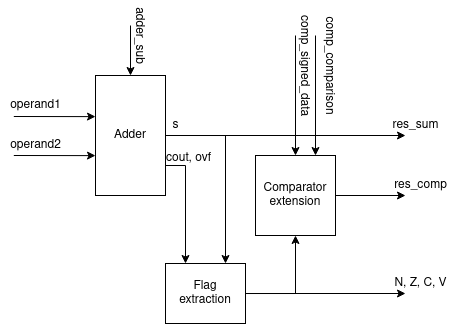
\includegraphics[width=0.6\textwidth]{./2-implementation/images/comparator.png}
	\caption{Schematic of the comparator implemented as an extension of the adder}
	\label{fig:comparator}
\end{figure}

It internally computes all of the possible comparisons and a multiplexer selects the result to output. In particular,
\begin{align*}
    lt &= N \texttt{ xor } \texttt{overflow} \\
    le &= lt \texttt{ or } Z \\
    eq &= Z \\
    ge &= \texttt{not } lt \\
    gt &= \texttt{not } le
\end{align*}
The \signal{overflow} signal is either \signal{C} or \signal{V},
depending on whether the comparison should consider its operands as respectively unsigned or signed.

It is clear to see how it is the controller's job to correctly deliver all of the necessary commands when a comparison
is requested, such as switching the adder to subtracting mode, deciding whether the operands are signed or not and
selecting the output.

\subsubsection{ALU Controller}
The controller for the ALU receives an ALU opcode to choose what operation to perform and then internally manages all
the necessary signals. It is described with a simple process and a switch on the opcode that updates the control
signals, as in any classical control unit output process.

For example, when the opcode is \texttt{alu\_op\_lt}, the control unit sets \texttt{adder\_sub} to 1 (to perform a
subtraction instead of an addition), switches the ALU multiplexer to select the comparison result, specifies to the
comparator that the data is signed and switches its multiplexer to choose the \texttt{lt} result.

All of the control signals are packed inside of a VHDL record to simplify possible future changes without the need of
modifying any entity in the circuit.

\subsection{Execution Controller and Input Selection}
Depending on the instruction to be executed, different sources for the two operands may be needed. Overall, the
execution stage receives the following signals:
\begin{itemize}
    \item Two entries from the register file
    \item Immediate
    \item Program counter
    \item Data from the Memory stage (used in forwarding)
    \item Data from the Write-Back stage (used in forwarding)
\end{itemize}
To these, some constants are inserted as additional options, such as the constant 0 being used in various operations.
The two operands which are fed to the ALU are selected from the EXController. In order to
pick the operands, it analyses three control signals: \texttt{instruction\_type} from the Control Unit and the two
\texttt{sel\_forward} from the Forward Unit.

The control logic works as follows: first, \texttt{instruction\_type} is analysed. This signal specifies what kind of
operators the current instruction works with, specifically if each one is a register, a specific constant,
the immediate and so on.
Whenever an operand is not a register, this request is immediately accepted and the corresponding
operand is selected since there are no risks of hazards. Whenever one operand is a register, instead, hazards are
a risk and the signals from the forwarding unit should be considered as well.

The candidates for operand 1 and 2 are not necessarily the same, so they are categorized in a generic way that allows
all the supported instructions to be executed but still optimizes the selection process. The multiplexers for the two
operands may then be connected to the specific signals associated to the generic selector.
All of the possible values for both operands are listed in \autoref{tab:exe-operands}.

\begin{table}[htbp]
    \center
    \begin{tabular}{|l|l|l|}
        \hline
        Selector               & Operand 1 value           & Operand 2 value           \\ \hline
        \texttt{SEL\_ZERO}     & 0                         & 0                         \\ \hline
        \texttt{SEL\_OPERAND}  & Register 1                & Register 2                \\ \hline
        \texttt{SEL\_CONST}    & 0                         & 4                         \\ \hline
        \texttt{SEL\_SPECIAL}  & PC                        & Immediate                 \\ \hline
        \texttt{SEL\_FWD\_MEM} & Data from Memory stage    & Data from Memory stage    \\ \hline
        \texttt{SEL\_FWD\_WB}  & Data from Write-Back stage & Data from Write-Back stage \\ \hline
    \end{tabular}
    \caption{Possible operand values for both operands in the Execution stage}
    \label{tab:exe-operands}
\end{table}
